\documentclass{article}

\usepackage{xcolor}
\usepackage{graphicx}
\usepackage{mathptmx}
\renewcommand\familydefault{\rmfamily}

\title{Final Assignment}
\author{Ehsan Abdollahi Nasab}
\date{\today}

\begin{document}

    \maketitle

    \section{Git and GitHub}
    \subsection{Repository Initialization and Commits}
    \textbf{Write about how you set up the repository for this assignment. Explain every step in detail.}
    {\color{green}
    For this I used GitHub website. I chose "Create New..." then "New Repository". After that I set the Repository; named it "FinalAssignment", chose it to be "Public" and add a "README file"
    \color{black}.}
    \subsection{GitHub Actions for LaTeX Compilation}
    \textbf{Provide a walkthrough of setting up GitHub Actions to automatically compile your LaTeX document and any challenges you encountered.}
    {\color{green}
    \color{black}}

    \section{Exploration Tasks}
    \subsection{Vim Advanced Features}
    \textbf{Explore and document 3 advanced features of Vim that were not covered in class.}
    {\color{green}
    \begin{itemize}
        \item \textbf{Change-list jumps:} helps in iterating through recent cursor positions (where changes were made)
        \texttt{g;} go to the previous position of cursor in change list
        \texttt{g,} go to the next position of cursor in change list
        \item \textbf{Marks:} Marks allow us to label cursor position. It can be used to label import locations in file for easy navigation.
        \texttt{m<char>} set label \textlesschar\textgreater to current cursor position
        \texttt{`<char>} go to position labeled \textlesschar\textgreater
        \item \textbf{Tags:} Tags are also labels used for jumping through them. Tags are read from the tags file.
        Important keys:
        \texttt{tag <tagname>} position the cursor on tag \texttt{<tagname>} position
        \texttt{CTRL-T} go back after the previous jumps
        \textt{:ptag <tagname>} show tag in the preview window (see :help preview-window)
        \texttt{CTRL-W z} close preview window (opened by above 2 commands)
    \end{itemize}
    \color{black}
    }
    \subsection{Memory Profiling}
    \subsubsection{Memory Leak}
    \textbf{In short, explain what memory leaks are and how they might happen in your program.}
    {\color{green}
        It happens when a computer program poorly handles memory allocations and fails to free up the memory that is no longer required
    \color{black}.}
    \subsubsection{Memory Profilers}
    \textbf{Read about a tool called Valgrind and write about their purpose and how it helps when memory leaks happen.}
    {\color{green}
        Valgrind is an instrumentation framework for building dynamic analysis tools.
    \color{black}}

    \section{GNU/Linux Bash Scripting}
    \subsection{fzf}
    \textbf{What is fuzzy searching? Give a short description.}
    {\color{green}
        A fuzzy search is a technique that uses search algorithms to find strings that match patterns approximately. It's particularly useful for helping users find webpages without having to know exactly what they're looking for or how a word is spelled
    \color{black}.}
    \textbf{Install fzf on your machine and give a description of what the following command does:
    \texttt{ls | fzf}}
    {\color{green}
        lists all files and directories.
        Pipes this list into fzf.
        Opens an interactive interface where you can filter the list of files. As you type, fzf narrows down the options based on your input.
        Once you find the file or directory you want, you can select it
    \color{black}}
    \subsection{Using fzf to find your favorite PDF}
    \textbf{You might have came across moments when you want to open up a certain PDF when studying for your final exams but finding the directory of that PDF is a very gruesome and tiring process. In this section, we will be using fzf to find our PDF in seconds! We will be going step by step on how to find your file and use fzf to select it.
    \begin{enumerate}
        \item We first need to list the directory of all the files with the extension .PDF. Write a command to list the directory of all the files with the extension .PDF
        \textcolor{green}{\texttt{fd -e pdf}}
        \item Now we have to select the PDF we want using fzf. Write a command to use fzf to select a PDF from the data we gathered above.
        \textcolor{green}{\text{fd -e pdf | fzf}}
    \end{enumerate}}
    \subsection{Opening the file using Zathura}
    \textbf{Now that have selected which PDF we want to open, we can use a very minimalistic program called Zathura to open it. Write a command that uses the commands above to open the file using Zathura.}

    \section{Git \& FOSS}
    \subsection{Issues}
    \textbf{Create a sample issue in the repository below and attach its screenshot in your LaTeX document: https://github.com/MiliAxe/CW-Final}
    \begin{figure}[h]
        \centering
        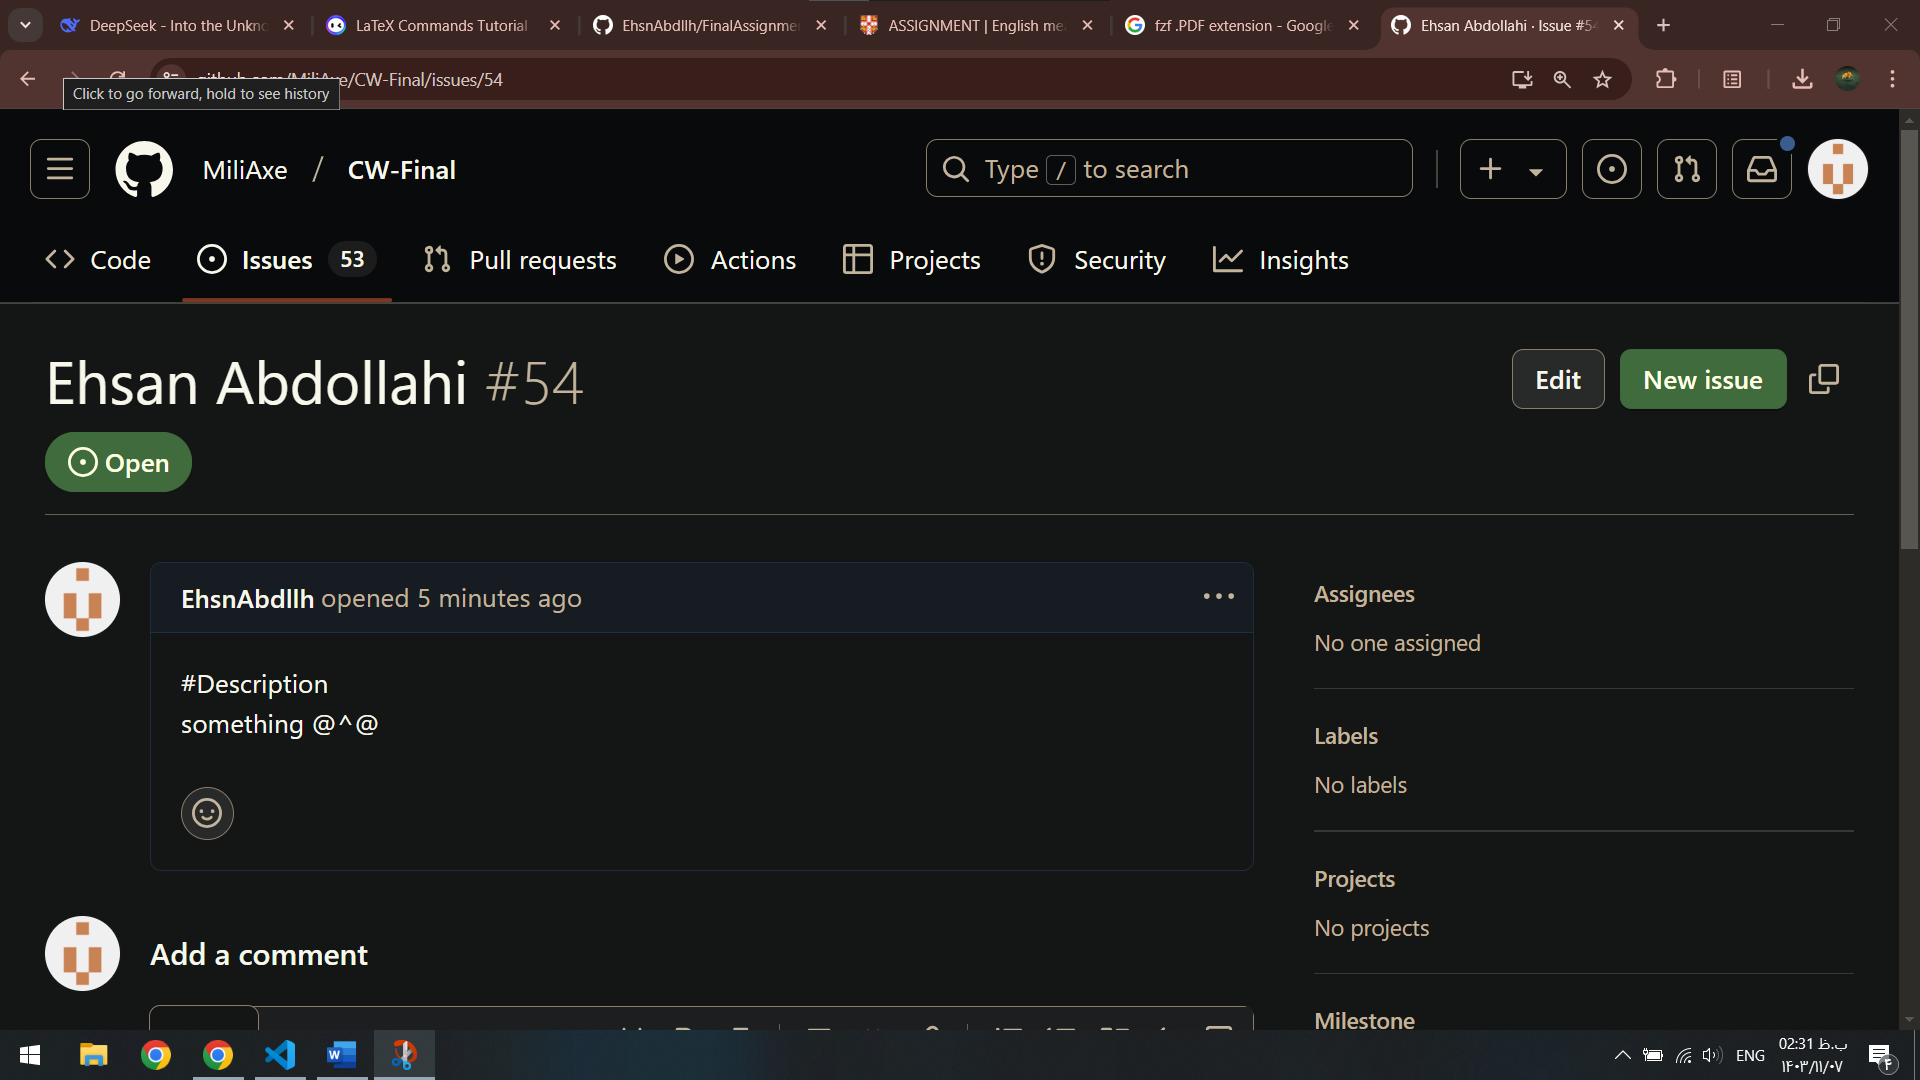
\includegraphics[width=1\textwidth]{Screenshot.png}
        \caption{my issue in GitHub website}
        \label{fig:my_image}
    \end{figure}
    \subsection{FOSS contribution}
    \textbf{Do you see yourself contributing to FOSS projects in the future? If yes, what kind of projects are you interested in contributing to? If no, why not?}

\end{document}